\documentclass[11pt]{article}
\usepackage[italian]{babel}
\usepackage[utf8]{inputenc}
\usepackage{graphicx}
\usepackage{float}
\usepackage{amsmath}
\usepackage{amsfonts}
\usepackage{hyperref}
\usepackage{verbatim}
\usepackage{glossaries}
\usepackage{dirtytalk}
\usepackage{wrapfig}


\usepackage[normalem]{ulem}
\newcommand{\code}[1]{\texttt{#1}}
\newcommand{\numpy}{{\tt numpy}}    % tt font for numpy
\topmargin -.5in
\textheight 9in
\oddsidemargin -.25in
\evensidemargin -.25in
\textwidth 7in
\begin{document}

% ========== Edit your name here
\author{Simone Montali\\monta.li}
\title{Riassunti di Crittografia - Tecnologie Internet}

\maketitle

\medskip
\section{Concetti generali}
Prima di tutto, definiamo il significato di \textbf{computer security}: la protezione applicata ad un sistema informativo con lo scopo di ottenere integrità, disponibilità e confidenzialità delle risorse. Emerge un concetto molto importante: la \textbf{CIA triad}, ossia confidenzialità, integrità, availability. (ricordiamo però altri due obiettivi: autenticità e accountability).
\subsection{CIA Triad}
\subsubsection{Confidentiality}
La confidentiality ha l'obiettivo di preservare restrizioni sull'accesso alle informazioni, inclusa la privacy personale ed informazioni proprietarie. Con \textbf{data confidentiality} intendiamo che informazioni confidenziali non sono rese visibili ad individui non autorizzati. Con \textbf{privacy} intendiamo che ogni individuo decide quali informazioni che lo riguardano rendere disponibili, e a chi. 
\subsubsection{Integrity}
L'integrity protegge dalla modifica o distruzione di informazioni, includendo non-repudiation e authenticity. Una perdita di integrity è la modifica non autorizzata di informazioni. Con \textbf{data integrity} intendiamo l'assicurarsi che informazioni e programmi vengano cambiati in maniera definita. Con \textbf{system integrity} intendiamo l'assicurarsi che un sistema svolga le sue funzioni in maniera corretta, libero da manipolazioni. 
\subsubsection{Availability}
Con availability intendiamo l'accesso affidabile alle informazioni. Una perdita di availability è l'interruzione dell'accesso ad alcune risorse.
\subsubsection{Authenticity}
Con authenticity intendiamo la proprietà, delle informazioni, di essere genuine e verificabili. In pratica, la verifica che gli utenti siano chi dicono di essere.

\subsubsection{Accountability}
Il goal dell'accountability è quello di poter tracciare tutte le azioni di un'entità sul sistema, in modo da riconoscere i colpevoli di un eventuale security breach. 

\subsection{Sfide della computer security}
Elenchiamo ora alcune sfide a cui la computer security deve sopperire:
\begin{enumerate}
    \item I requirements di sicurezza sembrano semplici, ma i meccanismi per risolverli sono complessi
    \item Nello sviluppo di un meccanismo/algoritmo di sicurezza, bisogna sempre considerare i potenziali attacchi
    \item Per il punto precedente, spesso le procedure necessarie sono controintuitive
    \item Dopo aver progettato i sistemi di sicurezza, bisogna decidere dove utilizzarli
    \item I meccanismi di sicurezza coinvolgono spesso più di un algoritmo/protocollo
    \item Il vantaggio per un malintenzionato è chiaro: a lui basta trovare una sola falla, mentre il progettista deve coprirle tutte
    \item C'è una naturale tendenza da parte di utenti/manager a non notare i benefici della sicurezza finché è troppo tardi 
    \item La sicurezza richiede monitoring costante e regolare
    \item La sicurezza è spesso un aggiunta successiva alla progettazione, piuttosto che parte integrante
    \item Molti utenti/amministratori vedono la sicurezza come un impedimento alle operazioni
\end{enumerate}
\subsection{OSI security architecture}
Definiamo alcuni termini:
\paragraph{Security attack} Ogni azione che compromette la sicurezza delle informazioni possedute da un'organizzazione
\paragraph{Security mechanism} Un processo progettato per rilevare, prevenire e recuperare attacchi di sicurezza
\paragraph{Security service} Un servizio che migliora la sicurezza del data processing/transfer di un'organizzazione. Sono progettati come antagonisti degli attacchi di sicurezza, e fanno utilizzo di meccanismi di sicurezza
\paragraph{Threat} Il potenziale per una violazione di sicurezza, che esiste quando c'è una circostanza, possibilità, azione o evento che potrebbe mettere a rischio la sicurezza.
\paragraph{Attack} Un assalto alla sicurezza di sistema che deriva da un intelligent threat, ossia un tentativo deliberato di evadere i sistemi di sicurezza.
\subsection{Security attacks}
Gli \textbf{attacchi attivi} coinvolgono qualche modifica del data stream, mentre quelli passivi sono di 4 tipi:
\begin{itemize}
    \item \textbf{spoofing}: attacca l'authenticity
    \item \textbf{tampering}: attacca l'integrity 
    \item \textbf{replay/reflection}: attacca l'authenticity
    \item \textbf{Denial Of Service}: attacca l'availability
\end{itemize}
È difficile prevenire gli attacchi attivi perché il numero di vulnerabilità è troppo alto: il goal è minimizzarne i danni. 
\subsection{Security service}
Un \textbf{security service} è un servizio di comunicazione/processing fornito da un sistema per dare specifici tipi di protezione a risorse; implementa security policies ed è implementato da security mechanisms. Fornisce diverse tipologie di sicurezza.
\subsubsection{Confidentiality}
Protezione verso accesso ai dati non autorizzato. È collegato a dati ed anonimità.
\subsubsection{Data integrity e message authentication}
La data integrity è la proprietà che i dati non siano stati cambiati, distrutti o persi. Protegge contro modifiche non autorizzate, rilevando cambiamenti. La data origin authentication certifica la fonte di un dato, verificandone l'identità. La message authentication è l'insieme delle due cose.
\subsubsection{Peer entity authentication}
Fornisce la conferma dell'identità di un peer in un'associazione. Due entità sono considerate peers se implementano lo stesso protocollo in sistemi diversi. L'authentication è utilizzata nello stabilimento della connessione o durante il trasferimento. Prova a fornire anche l'assicurazione che un'entità non sia mascherata o stia replicando una connessione passata.

\subsubsection{Authorization e access control}
L'authorization è la verifica dei permessi su una risorsa/sistema. L'access control è l'abilità di limitare e controllare l'accesso ad un sistema. 
\subsubsection{System integrity and availability}
La system integrity è la qualità che un sistema ha quando può eseguire la sua funzione. Si ottiene proteggendo il sistema da modifiche, perdite, distruzione. L'availability è la proprietà di un sistema di essere accessibile ed utilizzabile quando necessario, concordando con le specifiche della performance del sistema. 
\subsubsection{Accountability e non-repudiation}
L'accountability è la proprietà di un sistema/risorsa che assicura che le azioni di un'entità siano tracciabili a quell'entità. L'\textbf{audit} è un sistema che salva informazioni necessarie all'accountability.
La non-repudiation fornisce protezione verso il falso rinnego di azioni. 
\subsection{Meccanismi di sicurezza}
I meccanismi di sicurezza hanno relazioni coi servizi; citiamo:
\begin{itemize}
    \item Cifratura
    \item Firma digitale
    \item Access control
    \item Verifica dell'integrità dei dati
    \item Scambio di autenticazione
    \item Traffic padding
    \item Routing control
    \item Notarization
\end{itemize}
\subsection{Principi di security design}
Elenchiamo alcuni principi di security design:
\paragraph{Economy of mechanism} Significa che il design di misure di sicurezza dovrebbe essere il più semplice possibile.
\paragraph{Fail-safe defaults} Il concetto è basarsi sui permessi, piuttosto che l'esclusione. La situazione di default è mancanza di accesso.
\paragraph{Complete mediation} Significa che ogni accesso deve essere verificato tramite il meccanismo di access control.
\paragraph{Open design} Mentre le encryption keys devono essere segrete, gli algoritmi devono essere pubblici.
\paragraph{Separazione di privilegi} Attributi di privilegio multipli sono necessari per l'accesso ad una risorsa restricted.
\paragraph{Least privilege} Ogni processo deve operare con il numero più basso di permessi possibile.
\paragraph{Least common mechanism} Il design deve minimizzare le funzioni utilizzate da più utenti, fornendo sicurezza mutual.
\paragraph{Psychological acceptability} I meccanismi di sicurezza non devono interferire con il lavoro degli utenti. (least astonishment)
\paragraph{Isolation} È un principio che si applica a tre contesti: 
\begin{enumerate}
    \item Sistemi di accesso pubblici, che devono essere isolati da risorse critiche
    \item Processi e file di utenti individuali devono essere isolati gli uni gli altri 
    \item I meccanismi di security devono essere isolati: non dev'essere possibile accedervi
\end{enumerate} 
\paragraph{Modularity} Si riferisce al separamento delle funzioni di sicurezza in moduli, ed all'architettura modulare per il design.
\paragraph{Layering} Si riferisce all'utilizzo di approcci multipli di protezione indirizzati a persone, tecnologia, operazioni.
\subsection{Attack surface e trees}
Un'\textbf{attack surface} consiste nelle vulnerabilità raggiungibili di un sistema. Un \textbf{attack tree} è una struttura gerarchica ad albero che rappresenta le tecniche di exploit delle vulnerabilità. 
\subsection{Modello per la network security}
Tutte le tecniche di sicurezza hanno due componenti: una trasformazione sulle informazioni, e un segreto condiviso. Consideriamo 4 tasks semplici per il design di un servizio:
\begin{enumerate}
    \item Progettare un algoritmo per la trasformazione 
    \item Generare l'informazione segreta
    \item Sviluppare metodi per la distribuzione e condivisione del segreto
    \item Specificare un protocollo utilizzabile dalle entità che partecipano all'algoritmo
\end{enumerate}
\section{Secret Key Cryptography}
Introduciamo anzitutto il concetto di \textbf{crittografia}: studio ti tecniche matematiche relative alla sicurezza informatica, in presenza di avversari. Il messaggio originale è detto \textbf{plaintext}, quello codificato \textbf{ciphertext}. Il processo di conversione da plaintext a ciphertext è detto deciphering o decryption. Uno schema utilizzato per l'encryption è detto cryptographic system o cipher.
Nella \textbf{secret key cryptography} abbiamo una secret key, valore indipendente dal plaintext e dall'algoritmo, che produce un output differente in base alla chiave.
I sistemi crittografici sono caratterizzati da 3 dimensioni: la tipologia di operazioni, il numero di chiavi, il modo di processamento del plaintext.
Le tecniche utilizzate per decifrare un messaggio senza conoscenza dei dettagli di cifratura cadono nell'area della \textbf{cryptanalysis}. Questo tipo di attacco esploita le caratteristiche dell'algoritmo per tentare di dedurre un plaintext. In un \textbf{attacco brute force} l'attaccante prova ogni chiave possibile finché non ottiene il plaintext. Un \textbf{side channel attack} è un attacco basato su informazioni ottenute dall'implementazione fisica del sistema, piuttosto che da debolezze dell'algoritmo. 
\subsection{Tipi di attacco}
\subsubsection{Ciphertext only}
Il malintenzionato ha visto e salvato del ciphertext analizzabile, e può riconoscere quando ha ottenuto il plaintext. È l'attacco più difficile, è necessario abbastanza ciphertext e si hanno poche informazioni.
\subsubsection{Known plaintext attack}
L'opponent conosce una coppia (plaintext, ciphertext), dalla quale prova ad ottenere le corrispondenze. Il plaintext viene ottenuto anche tramite certe keywords, pattern, probable-words. 
\subsubsection{Chosen plaintext/ciphertext attack}
L'opponent può scegliere ogni plaintext e criptarlo tramite il sistema.

\subsection{Computational e unconditional security}
Uno schema di encryption è detto \textbf{computationally secure} se: il costo per rompere il cipher è più alto del valore dell'informazione, e il tempo necessario è più lungo del lifetime dell'informazione. 
Uno schema è detto \textbf{unconditionally secure} se il ciphertext generato dallo schema non contiene abbastanza informazioni per determinare il plaintext corrispondente, non importa quanto ciphertext sia disponibile. 
\subsection{Tecniche di encryption classiche}
Distinguiamo tra tecniche di substitution e transposition. 
\subsubsection{Cifrario di Cesare}
Il primo utilizzo di cifrario. Si shiftano le lettere di un indice k.
\begin{displaymath}
    C = E(k,p) = (p+k) \textrm{mod}26
\end{displaymath}
\subsubsection{Monoalphabetic ciphers}
Basati su permutazioni dei caratteri alfabetici. Ci sono $26!$ possibili chiavi. Però, l'opponent ha un'altra linea di attacco: exploitare le regolarità del linguaggio, come la frequenza delle lettere o i digrams.
\subsubsection{Multiletter ciphers}
Il multiletter cipher più conosciuto è il \textbf{Playfair}, che tratta i digrams come singole unità e le traduce in digrams del ciphertext. Il Playfair è basato sull'uso di una matrice 5x5 di lettere, costruita con una keyword. 
\subsubsection{Polyalphabetic ciphers}
Un altro modo di migliorare i cifrari monoalfabetici è utilizzare differenti sostituzioni monoalfabetiche in ordine. Un esempio è il \textit{Vigenère cipher}, nel quale abbiamo un vettore di chiavi da sommare ai caratteri (come in Cesare). La lunghezza della chiave può però essere ricavata dalle ripetizioni: se due sequenze identiche di lettere di plaintext si ripetono a una distanza multipla della chiave, genereranno ciphertext identici. 
\subsubsection{One-time pad}
Citiamo il \textit{Vernam cipher}, in cui abbiamo un vettore di chiavi lungo quanto il plaintext. Se il vettore è veramente random, otteniamo il cosiddetto \textbf{one-time pad}: non c'è relazione statistica tra ciphertext distinti, e sarà quindi unconditionally secure.
\subsubsection{Row transposition ciphers}
In questi cifrari, scriviamo il messaggio in un rettangolo, riga per riga, e leggiamo ogni colonna, con ordine definito dalla chiave. Possiamo anche effettuare più stadi di trasposizione. 
\subsubsection{Product ciphers}
I cipher che utilizzano sostituzioni o trasposizioni potrebbero non essere abbastanza sicuri. Consideriamo quindi di utilizzare più ciphers in successione, ad esempio una sostituzione seguita da trasposizione. 
\subsubsection{Block e stream cipher}
Uno \textbf{stream cipher} encrypta uno stream un bit/byte alla volta. Un \textbf{block cipher} cripta invece un blocco di plaintext alla volta, ottenendo un blocco di ciphertext, solitamente di lunghezza 64/128 bit. Un \textbf{ideal block cipher} è un cifrario arbitrario di sostituzioni reversibili. Non è pratico dal punto di vista implementativo/delle performance. Il mapping stesso costituisce la chiave, che ha quindi lunghezza $n2^n$ bits. 
\subsubsection{Feistel cipher}
\begin{wrapfigure}{r}{0.25\textwidth}
    \begin{center}
      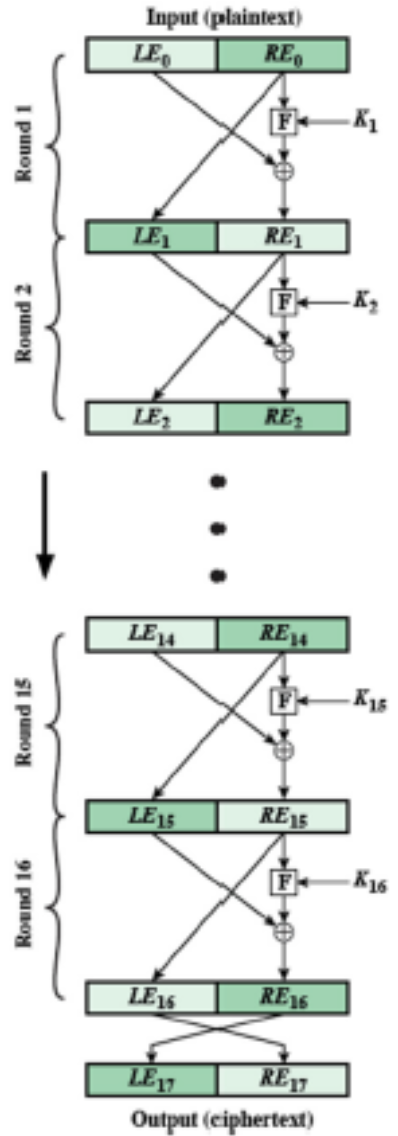
\includegraphics[width=0.24\textwidth]{res/crypto/Feistel.png}
    \end{center}
    \caption{Feistel encryption}
  \end{wrapfigure}
Feistel propose di approssimare l'ideal block cipher utilizzando il concetto di product cipher, ossia l'esecuzione di più cifrari in sequenza: sviluppiamo un block cipher con key length di $k$ bits, e block length di $n$ bits, rendendo possibili $2^k$ trasformazioni, piuttosto che $2^n!$. In particolare, Feistel propose l'uso di un cifrario che alternasse sostituzioni (ogni elemento del plaintext è sostituito da un elemento corrispondente del ciphertext) e permutazioni (una sequenza di elementi del plaintext è sostituito dalla sua permutazione). Questo cifrario è l'applicazione pratica di una proposta di Claude Shannon, che consisteva nell'alternare confusione e diffusione:
\begin{itemize}
    \item Nella \textbf{diffusione}, la struttura statistica del plaintext è dissipata in statistiche long-range del ciphertext. Questo è ottenuto facendo in modo che ogni cifra del plaintext influenzi più cifre del ciphertext.
    \item La \textbf{confusion} cerca di rendere complessa la relazione tra le statistiche del ciphertext e il valore dell'encryption key, tramite un complesso meccanismo di sostituzione 
\end{itemize}
Gli input all'algoritmo così generato sono un plaintext block di lunghezza $n=2w$ bits ed una chiave $K$. Il plaintext block è diviso in due metà: $LE_0$ e $RE_0$, che passano più stadi di processamento e vengono poi combinati. 
Il processo di decryption è essenzialmente lo stesso: basta invertire l'ordine delle chiavi.
Possiamo variare alcuni parametri per modificare le caratteristiche del cifrario:
\begin{itemize}
    \item Un \textbf{block size} maggiore aumenta la sicurezza. Valori tipici sono 64/128 bits.
    \item Una \textbf{key size} maggiore incrementa la security. 128 bits è la dimensione classica.
    \item Aumentare il \textbf{numero di rounds} rende più difficile la cryptanalysis.
    \item Un \textbf{algoritmo di generazione di subkeys} più complesso aumenta la difficoltà della cryptanalysis
    \item Aumentare la complessità della funzione di arrotondamento $F$ aumenta la resistenza alla cryptanalysis
\end{itemize}
\subsection{DES}
DES, \textit{Data Encryption Standard} fu creato nel 1977 dal NIST. L'algoritmo è detto \textbf{DEA} (\textit{Data Encryption Algorithm}), che è un cifrario Feistel con blocchi da 64 bit e chiavi da 56 bit. Nel 1999 il NIST lancia TDEA, detto anche 3DES (\href{https://www.facebook.com/IPIUBELLELLIDIPARMA/videos/vl.2430501220562185/1326509910720610/?type=1}{\textit{In do ela al 3DES?}}). 
\subsubsection{Funzionamento}
L'encryption è composta di 4 fasi principali:
\begin{itemize}
    \item Prima di tutto, \textbf{key transformation} per ottenere 16 chiavi 48-bit da quella principale a 56-bit
    \item Initial Permutation ($IP$)
    \item 16 round identici di confusione-diffusione con la chiave 
    \item Permutazione finale ($IP^{-1}$)
\end{itemize}
Otteniamo così l'effetto valanga: una piccola modifica nel plaintext o la chiave produce una modifica significativa nel ciphertext. La decryption usa lo stesso algoritmo con le subkeys al contrario.
\subsubsection{Vantaggi di DES}
DES ha 3 vantaggi principali: le chiavi a 56-bit rendono il bruteforce poco pratico, nessuno ha ancora trovato debolezze nell'algoritmo, resiste ai timing attacks. 
\subsubsection{Double DES}
Con double DES, dato un plaintext P e due chiavi $K_1$ e $K_2$, il ciphertext è generato come
\begin{displaymath}
    C=E(K_2, E(K_1,P))
\end{displaymath}
Questo algoritmo è però suscettibile ad attacchi \textbf{meet-in-the-middle}, basato sull'osservazione che
\begin{displaymath}
    X=E(K_1, P) = D(K_2, C)
\end{displaymath}
Data una coppia $(P,C)$, criptiamo P per tutti i possibili valori di $K_1$, salviamo i risultati in una tabella e li ordiniamo per X. Poi, decriptiamo C usando tutti i possibili valori di $K_2$, controllando la tabella. In caso di match, testiamo le due chiavi contro un'altra coppia $(P,C)$ conosciuta. 
\subsubsection{3DES}
Distinguiamo tra 3DES a 2 chiavi e a 3 chiavi. Nel primo,
\begin{displaymath}
    C=E(K_1,D(K_2, E(K_1,P)))\hspace{10px}P=D(K_1, E(K_2, D(K_1,C)))
\end{displaymath}
A 3 chiavi, invece:
\begin{displaymath}
    C=E(K_3,D(K_2, E(K_1,P)))\hspace{10px}P=D(K_1, E(K_2, D(K_3,C)))
\end{displaymath}
\subsection{AES}
AES, \textit{Advance Encryption Standard} fu pubblicato da NIST nel 2001. È conosciuto anche come Rijndael block cipher, ed è adottato dal governo americano.
La struttura generale vede block size di 128 bits, dipinti in una matrice 4x4 di bytes. Il blocco è copiato ad un array \textbf{State}, modificato ad ogni stadio dell'encryption. La chiave è espansa in un array di parole da 4 bytes. Il cifrario consiste di $N$ round, dipendente dalla key length. I primi $N-!$ rounds consistono di 4 trasformazioni: SubBytes (usa un S-box per eseguire sostituzioni byte-a-byte), ShiftRows (permutazione semplice), MixColumns(sostituzione che usa l'arithmetic over $GF(2^8)$), AddRoundKey(XOR bitwise del blocco con una porzione della chiave espansa). La trasformazione iniziale è una AddRoundKey, l'n-simo round contiene 3 trasformazioni. Encryption e decryption hanno struttura semplice ma leggermente diversa. AddRoundKey è l'unico stadio che coinvolge anche la chiave (cifrario Vernam). 
\subsubsection{Aritmetica dei finite fields}
Un finite field è un field con numero finito di elementi (ordine del field). Un finite field di ordine m esiste solo se $m=p^n$ per qualche intero positivo $n$ e intero primo $p$.
Il finit field fi ordine $p^n$ è denotato $GF(p^n$) (Galois Field). Gli elementi sono rappresentati come polinomiali con coefficienti binari. L'addizione è svolta tramite il bitwise XOR delle due stringe di coefficienti a n-bit. La moltiplicazione con il modulo. L'inverso è definito come $1 mod P(x)$. AES opera su byte a 8 bit. Tutte le operazioni sono svolte sul field finito $GF(2^8)$ con il polinomiale irriducibile $m(x) = x^8 + x^4 + x^3 + x + 1$. Ci sono 30 possibili polinomi irriducibili. 
\subsubsection{Operazioni}
\paragraph{SubBytes} Il SubBytes è l'operazione di sostituzione in avanti dei byte: una semplice lettura da tabella. Ogni byte dello State è mappato in un altro. L'InvSubBytes è lo stesso processo con un inverse S-box.
\paragraph{ShiftRows} La trasformazione in avanti di shifting delle row esegue degli shift circolari sulla seconda, terza e quarta riga dello State. L'InvShiftRows fa la stessa cosa nella direzione inversa.
\paragraph{MixColumns} La trasformazione di mix delle colonne in avanti opera su ogni colonna individualmente. Ogni byte di una colonna è mappata in un nuovo valore, che è funzione di tutti i 4 bytes della colonna. È, insomma, una moltiplicazione tra matrici.
InvMixColumns è definita da una diversa moltiplicazione tra matrici.
\paragraph{AddRoundKeys} Nella trasformazione add round key in avanti, i 128 bit dello State vengono XORrati (bitwise) con i 128 bit della round key. L'inversa è uguale identica: lo XOR è inverso.
\paragraph{Key expansion} La key expansion prende in input una chiave a 16 byte (4 parole) e produce un array lineare di parole. In AES128 l'array ha 44 elementi. 

\subsubsection{Sicurezza di AES}
Il brute force è improbabile: già solo con chiavi a 128 bit, abbiamo $3.4 x 10^38$ chiavi possibili. 
\subsection{Metodi di encrypting di grandi messaggi}
Solitamente, abbiamo una quantità di dati arbitraria. NIST ha pubblicato 5 modalità: ECB, CBC, OFB, CFB, CM. A volte è necessario del padding per raggiungere una lunghezza specifica: bit padding (1 poi 0 necessari), ANSI X.923 (ultimo byte che definisce lunghezza del padding, gli altri 0), RFC 5652 (ogni byte contiene la lunghezza del padding). 
\subsubsection{Electronic Code Book}
ECB rompe il messagio in $n$ blocchi di dimensione $b$ con padding per l'ultimo. Ogni blocco è criptato indipendentemente con chiave $K$. ECB è molto semplice e non introduce operazioni extra, ma potrebbero apparire ripetizioni, è vulnerabile alle similarities tra ct e agli attacchi con conoscenza parziale del plaintext.
\subsubsection{Cipher Block Chaining}
CBC utilizza un Initialization Vector per fare in modo che due blocchi uguali diano ct diversi. Ha decryption semplice, ct dipendente da tutti i messaggi precedenti, ottime performance. Però, un valore IV costante potrebbe portare a problemi.
\subsubsection{Output FeedBack}
Anche in OFB, il ct è funzione del precedente plaintext, con una nonce. I vantaggi sono due: la sequenza pseudorandom può essere generata in anticipo, e c'è possibilità di criptare messaggi di lunghezza variabile. Però, dobbiamo usare sempre la stessa sequenza pseudorandom (come un OTP), e sender/receiver devono essere sincronizzati. 
\subsubsection{Cipher FeedBack}
In CFB il plaintext è diviso in segmenti di s bits, piuttosto che in blocchi. Come OFB, la sequenza può essere generata in anticipo, ma ha gli stessi problemi. 
\subsubsection{Counter Mode}
CM è simile a OFB, la sequenza di counter deve avere la proprietà di blocchi diversi tra loro. Ha vari vantaggi: le funzioni forward cipher possono essere applicate ai counter prima della disponibilità del plaintext, le funzioni di cipher possono essere eseguite in parallelo, il plaintext block che corrisponde a un ct può essere recuperato indipendentemente dagli altri. Ha, però, limitazioni: non dobbiamo usare mai la stessa counter sequence, e sender/receiver devono essere sincronizzati.
\subsection{Utilizzi principali della secret key cryptography}
La secret key cryptography ricopre soprattutto confidentiality e authentication: nella prima, possiamo trasmettere su un canale poco sicuro e salvare dati su storage poco sicuro. Per la seconda, possiamo autenticare utenti tramite un meccanismo challenge-response.
Abbiamo alcuni svantaggi: richiede sempre un metodo sicuro per lo scambio di chiavi, ed in caso di chiavi permanenti pre-shared il numero totale di chiavi per N users è $N(N-1)/2$, che è troppo.

\section{Funzioni di hash e autenticazione}
\subsection{Hash function}
Una funzione hash $H$ accetta un blocco di dati $M$, di lunghezza variabile, e produce un hash di lunghezza fissata di lavore $h=H(M)$. Una \textbf{cryptographic hash function} è un algoritmo per il quale è computazionalmente infattibile trovare: un oggetto che restituisca un hash arbitraria, due oggetti con lo stesso hash. Per queste proprietà, le hash sono utilizzate spesso per determinare se i dati sono cambiati. 
\subsubsection{Message authentication}
La message authentication assicura che i dati ricevuti siano esattamente come inviati. Quando una hash function viene utilizzata per fornire message authentication, il valore dell'hash è detto \textbf{message digest}. Se c'è un mismatch, il ricevitore sa che il messaggio è stato alterato. 
Scongiuriamo un attacco man in the middle proteggendo il valore hash del messaggio.
\subsection{Requisiti di sicurezza}
Definiamo la \textbf{preimage} di $h$ come $h=H(x)$. Una collisione accade quando abbiamo $x \neq y$ e $H(x)=H(y)$. Se permettiamo input di lunghezza arbitraria, il numero di preimage per hash è arbitrariamente grande.
Elenchiamo 7 requisiti:
\begin{itemize}
    \item \textbf{Variable input size}
    \item \textbf{Fixed output size}
    \item \textbf{Efficiency}: $H(x)$ è relativamente semplice da calcolare dato $x$
    \item \textbf{Preimage resistant}: dato un valore hash $h$, è infattibile trovare una $y$ tale che $H(y)=h$.
    \item \textbf{Second preimage resistant}: dato un blocco $x$, è computazionalmente infattibile trovare una $y \neq x$ con $H(y)=H(x)$.
    \item \textbf{Collision resistant}: è computazionalmente infattibile trovare $x \neq y$ con $H(x) = H(y)$
    \item \textbf{Pseudorandomness}: l'output di H è compatibile con i test standard per la pseudorandomness
\end{itemize}
Se le proprietà da 1 a 5 sono soddisfatte, si dice \textbf{weak hash function}, se anche la 6 la è abbiamo una \textbf{strong hash function}.
\subsection{Struttura generale di una secure hash function}
La struttura, proposta inizialmente da Merkle, è riferita ad un'iterated hash function. L'algoritmo di hash richiede l'uso ripetuto di una funzione di compressione $f$, che prende due input (un input a n-bit dallo step precedente e blocco a b-bit). Spesso, $b>n$. Il problema di progettare una secure hash function è principalmente quello di progettare una funzione di compressione collision-resistant.
\subsection{Secure Hash Algorithm}
SHA, pubblicato dal NIST, è la funzione di hash più utilizzata. Abbiamo diverse versioni, l'ultima uscita nel 2015 (SHA-3).
\subsubsection{SHA-1}
Qui, l'input message (padded) è frammentato in blocchi da 512 bit, composti da 16 parole $X_0,X_1...X_{15}$. L'algoritmo utilizza un internal state a 160 bit. Il suo valore per processare il primo blocco è sempre lo stesso. Dopo 80 round, l'internal state è utilizzato per processare il prossimo blocco. Quando i blocchi sono finiti, l'internal state è l'hash. Per ogni t-esimo round, deriviamo $W_t$ da $X_i$, utilizziamo una parola costante diversa $K_t$ tra 4 parole, utilizziamo una diversa funzione $F_t$ tra 4 (Ch, Parity, Maj, Parity). 
\subsubsection{SHA-2}
SHA-256 e SHA-512 sono calcolati con parole a 32 e 64 bit, rispettivamente, e hanno 64 e 80 round. SHA-224 e SHA-384 sono versioni troncate con valori iniziali diversi.
\subsubsection{SHA-3}
SHA-3 è comunemente chiamata Keccak. Supporta le stesse hash lengths di SHA-2. La sua struttura interna differisce significativamente dal resto della famiglia SHA, è una \textit{cryptographic sponge function}, ossia una funzione con input e output di lunghezza variabile, basata su una trasformazione a lunghezza fissa o permutazione che lavora su un numero fisso $b$ di bit (la larghezza). $f$ opera su uno state di $b=r+c$ bits, con $r$ detto bitrate e $c$ capacity. Di default in Keccak abbiamo $r=576$ bits e $c=1024$ bits. 
\subsection{Message Authentication Code (MAC)}
Un MAC è un checksum crittografico, generato da un algoritmo che crea un piccolo blocco di dimensione fissa, dipendente dal messaggio e da una chiave segreta K: $MAC=C_K(M)=C(K,M)$
Un MAC condensa un messaggio $M$ di lunghezza variabile ad un authenticator di lunghezza fissa, che è appeso a M come sua \textbf{signature}. Ha bisogno di non essere reversibile, ed è una funzione one-to-many: potenzialmente molti messaggi hanno lo stesso MAC, ma trovarli dev'essere difficile. 
\subsubsection{Data Authentication Algorithm}
DAA è un MAC basato su DES-CBC: utilizza $IV=0$ e zero-pad del blocco finale. Encrypta il messaggio utilizzando DES in modalità CBC, ed invia il blocco finale come MAC. 
\section{Public Key Cryptography}
La public key cryptography è probabilmente la rivoluzione più grande nella storia della crittografia. Gli algoritmi sono basati su funzioni matematiche, piuttosto che su sostituzione e permutazione. La caratteristica più importante è il suo essere \textbf{asimmetrica}, richiedendo l'uso di due chiavi (una pubblica, una privata). Siccome le implementazioni pratiche sono computazionalmente costose, la crittografia public-key è ristretta a due problemi principali: distribuzione delle chiavi e firma digitale. Le caratteristiche principali sono che: è computazionalmente infattibile determinare la chiave di decryption dato l'algoritmo e la chiave di encryption; una delle due chiavi può essere usata per l'encryption, l'altra per la decryption. 
\subsection{Public key cryptography per la confidentiality}
4 passi fondamentali:
\begin{enumerate}
    \item Ogni user genera un paio di chiavi utilizzate per l'encryption e la decryption.
    \item Ogni user rende disponibile la sua public key.
    \item Se Bob vuole inviare un messaggio confidential ad Alice, lo cripta con la chiave pubblica di Alice
    \item Quando Alice riceve il messaggio, lo decripta usando la sua chiave privata.
\end{enumerate}
\subsection{Public key cryptography per l'authentication}
In questo caso, Bob prepara un messaggio per Alice e lo cripta utilizzando la sua chiave privata. Alice può decriptarlo con la chiave pubblica di Bob, assicurandosi che l'abbia generato lui. In più, è impossibile modificare il messaggio senza accesso alla chiave privata. Per più efficienza, criptiamo un piccolo blocco di bit che sia funzione del documento.
\subsection{Requirements per la public key cryptography}
Un problema semplice è un problema risolvibile in tempo polinomiale come funzione della lunghezza dell'input. Un problema infeasible è un problema il cui costo di risoluzione cresce più velocemente di una funzione polinomiale, data la lunghezza dell'input. Solo pochi algoritmi sono stati accettati negli anni; tutti questi sono basati su una \textbf{trapdoor one-way function}, una famiglia di funzioni invertibili $f_k$ tali che $f_k(X)$ sia semplice, $X=f_k^{-1}(Y)$ sia semplice se conosciamo $k$ e $Y$, $X=f_k^{-1}(Y)$ sia infattibile se conosciamo solo Y.
\subsection{Cryptanalysis}
Distinguiamo 3 attacchi:
\begin{itemize}
    \item \textbf{Bruteforce}: la contromisura rispetto ai bruteforce è utilizzare chiavi di grandi dimensioni. 
    \item \textbf{Trovare la private data la public}: non è ancora stata provata l'impossibilità di questo attacco. 
    \item \textbf{Probable message attack}: sappiamo il messaggio probabile e la chiave, proviamo tutte le private.
\end{itemize}
\subsection{RSA}
In RSA il plaintext è criptato a blocchi aventi valore binario minore di $n$. Definiamo il blocco plaintext $M$ e il ct corrispondente $C$. Abbiamo:
\begin{displaymath}
    C=M^e mod n \hspace{10px}M=C^d mod n = (M^e)^d mod n = M^{ed}mod n
\end{displaymath}
Sia il sender che il receiver devono conoscere il valore di $n$. Il sender conosce il valore di $e$, e il receiver quello di $d$. Quindi, il receiver avrà public key $PU=\{e,n\}$ e private key $PR=\{d,n\}$. Il problema ora è: come ottenere $e,d,n$ tali che $M^{ed} mod n = M$ per tutti gli $M<n$? Prendiamo $p,q$ primi, e li teniamo segreti. Calcoliamo $n=pq$. Calcoliamo $\phi(n) = (p-1)(q-1)$ e lo teniamo segreto.
Poi scegliamo $e$, con $GCD(\phi(n),e) = 1$ e $1<e<\phi(n)$. Calcoliamo $d \equiv e^{-1} mod \phi(n)$ e lo teniamo segreto. 
Ora, sapendo $e$ ed $n$ ma non la trapdoor key $\phi(n)$, dovrebbe essere infattibile trovare $d$.
\subsubsection{Aspetti computazionali}
Sia l'encryption che la decryption di RSA necessitano l'elevamento di un intero a una potenza intera, mod n. Se l'elevamento fosse fatto sugli interi e poi modulato, i valori intermedi sarebbero enormi. Fortunatamente, possiamo sfruttare una proprietà dell'aritmetica modulare.
Per velocizzare RSA, si sceglie $e$ specificatamente, spesso 65537 ($2^{16}+1)$, 3 e 17. Non possiamo fare lo stesso con $d$: un valore $d$ piccolo è vulnerabile ai bruteforce e alla cryptanalysis.
Per prevenire la scoperta di $p$ e $q$ dobbiamo sceglierli da un insieme grande: serve un metodo per trovare numeri primi grandi, ed il più comodo è estrarre numeri casuali dispari e testarli. 
Avendo determinato $p$ e $q$, dobbiamo determinare $e$ e $d$: generiamo una serie di numeri random e li testiamo contro $\phi(n)$ finché un numero relativamente primo a $\phi(n)$ viene trovato, ossia $e$. Poi, $d$ viene calcolato tramite l'extended Euclid's algorithm.
\subsubsection{Possibili attacchi ad RSA}
Distinguiamo 5 attacchi possibili:
\begin{itemize}
    \item \textbf{Brute force}
    \item \textbf{Mathematical attacks}: fattorizzazione di n tramite GNFS (usando n>2048 bits si è al sicuro fino al 2030), o l'algoritmo di Shor's per quantum computers. Per evitare questi atttacchi, p e q devono differire poco in lunghezza, $(p-1)$ e $(q-1)$ devono contenere un fattore primo grande, $GCD(p-1,q-1)$ deve essere piccolo
    \item \textbf{Timing attacks}: controllando il tempo di decifratura si può ottenere la private key. Per mettersi al sicuro, constant exponentiation time, random delay, bilding (moltiplicazione ct per valore random)
    \item \textbf{Hardware Fault Based attacks}: grazie all'accesso fisico alla macchina, togliamo potenza al processore per produrre firme invalide da analizzare
    \item \textbf{Chosen Ciphertext Attack}: exploit di RSA in cui, scegliendo un blocco adatto, possiamo ottenere informazioni per la cryptanalysis. Per risolvere, modifichiamo il pt con optimal asymmetric encryption padding.
\end{itemize}

\subsection{Diffie-Hellman key exchange}
Vari prodotti commerciali utilizzano questa tecnica di scambio chiavi, proposta da Diffie ed Hellman nel 1976. Lo scopo è permettere a due utenti di scambiare chiavi per un utilizzo con secret key encryption. È meno generico di RSA: non fa encryption né firme. L'effettività è data dalla difficoltà del calcolo dei logaritmi discreti.
Una \textbf{primitive root} di un numero primo $p$ è una il cui modulo $p$ genera tutti gli interi da 1 a $p-1$.
Se $a$ è la primitive root del numero primo $p$, allora i numeri $a mod p, a^2 mod p,...$ sono interi distinti da 1 a $p-1$ in qualche permutazione. Per ogni intero $b$ e primitive root $a$ del numero primo $p$, possiamo trovare un esponente tale che $b \equiv a^i (mod p)$. L'esponente $i$ è detto \textbf{logaritmo discreto} di $b$ in base $a, mod p$.
Questo algoritmo è suscettibile ad attacchi man-in-the-middle.
\section{Digital Signatures}
\subsection{Principi delle firme digitali}
Il risultato più importante della public key cryptography è la firma digitale, che fornisce un set di capacità di sicurezza difficilmente implementabili in altro modo. La firma digitale permette di autenticare messaggi tramite una funzione secura di hashing come SHA-512. 
Per inviare un messaggio autenticato, gli appendiamo l'hash SHA, criptato con la chiave privata. In questo modo, il destinatario può calcolare l'hash del messaggio e vedere se l'hash coincide.
La firma digitale deve avere le seguenti proprietà:
\begin{itemize}
    \item Deve verificare l'autore, la data e l'ora della firma
    \item Deve autenticare i contenuti all'orario segnato
    \item Dev'essere verificabile da terze parti per risolvere dispute
\end{itemize}
L'autenticazione protegge due parti che scambiano messaggi, da parti terze malintenzionate.
\subsubsection{Tipi possibili di attacco}
Ci sono più possibilità di attacco:
\begin{itemize}
    \item \textbf{Key-only attack}: l'attacker conosce solo la chiave pubblica del mittente
    \item \textbf{Known message attack}: l'attacker ha un set di messaggi e le loro firme
    \item \textbf{Generic chosen message attack}: l'attacker ottiene firme valide da A, per messaggi che non dipendono dalla chiave pubblica di A
    \item \textbf{Directed chosen message attack}: simile a quello sopra, ma i messaggi vengono scelti in base alla chiave pubblica di A
    \item \textbf{Adaptive chosen message attack}: l'attacker richiede firme di messaggi che dipendono da quelle già ricevute
\end{itemize}
Elenchiamo anche i risultati ottenibili:
\begin{itemize}
    \item \textbf{Total break}: l'attacker ottiene la chiave privata
    \item \textbf{Universal forgery}: l'attacker trova un modo efficiente di costruire firme su messaggi arbitrari
    \item \textbf{Selective forgery}: l'attacker crea una firma per un particolare messaggio 
    \item \textbf{Existential forgery}: l'attacker crea una firma su un messaggio, non scelto da lui
\end{itemize}
\subsubsection{Requirements}
Abbiamo diversi requirements: la firma dev'essere un bit pattern dipendente dal messaggio, ed utilizzare informazioni conosciute al solo mittente. Dev'essere facile da costruire/verificare, ma non imitabile. Dev'essere inoltre facile da salvare.
\subsubsection{Digital Signature + Confidentiality}
La confidentiality può essere ottenuta criptando l'intero messaggio assieme alla firma, con una chiave segreta condivisa. È importante codificare l'insieme e non il solo messaggio prima della firma. In caso di dispute, una terza parte controlla il messaggio e la firma.
\subsection{Approcci alla firma digitale}
\subsubsection{Approccio RSA}
Nell'approccio RSA, il messaggio è hashato con risultato di lunghezza fissa. A questo punto, viene criptato l'hash utilizzando la chiave privata. Il destinatario riceve il messaggio e lo hasha, per verificare se coincide.
\subsubsection{Elgamal Digital Signature scheme}
Se $\alpha$ è una primitive root del numero primo $q$, abbiamo che i numeri $\alpha mod q, \alpha^2 mod q,...$ sono interi distinti da $1$ a $q-1$ in qualche permutazione. È dimostrabile che, se $\alpha$ è primitive root di $q$, per ogni intero $m$, $\alpha^m \equiv 1 (mod q)$ iff $m \equiv 1 (mod q-1)$, per ogni coppia di interi $i,j$, $\alpha^i \equiv \alpha^j (mod q)$ iff $i \equiv j (mod q-1)$.
L'utente genera una coppia di chiavi così:
\begin{enumerate}
    \item Genera un intero random $X_A$ tale che $1 < X_A < q-1$
    \item Calcola $Y_A = \alpha^{X_A} mod q$
    \item La chiave privata di $A$ è $X_A$, la pubblica $\{q,\alpha,Y_A\}$
\end{enumerate}
Il calcolo di $X_A$ da $Y_A$ è estremamente complesso, in quanto richiede la risoluzione di un logaritmo discreto.
Per firmare un messaggio $M$, l'utente $A$ computa l'hash $m=H(M)$, in modo che $m$ sia un intero $0 \le m \le q-1$. Poi forma la firma digitale così:
\begin{enumerate}
    \item Sceglie un intero $K$ tale che $1 \le K \le q-1$ e $GCD(K,q-1)=1$
    \item Calcola $S_1 = \alpha^K mod q$
    \item Calcola $K^{-1} mod (q-1)$
    \item Calcola $S_2 = K^{-1}(m-X_AS_1) mod (q-1)$
\end{enumerate}
Ogni utente può verificare così la firma:
\begin{enumerate}
    \item Calcola $V_1 = \alpha^m mod q$
    \item Calcola $V_2 = (Y_A)^{S_1}(S_1)^{S_2} mod q$
    \item La firma è valida se $V_1 = V_2$
\end{enumerate} 
\subsubsection{Schnorr Digital Signature Scheme}
Lo schema Schnorr minimizza la quantità di computazione necessaria per la generazione della firma: il lavoro principale non dipende dal messaggio e può essere fatto nell'idle time del processore. Il processo è basato sull'utilizzo di un numero primo $p$, con $p-1$ avente un fattore primo $q$ di dimensione appropriata. Tipicamente, $p$ è un numero a 1024-bit, e $q$ a 160 bit.
L'utente A genera una coppia di chiavi così:
\begin{enumerate}
    \item Sceglie i numeri primi $p$ e $q$, tali che $q$ sia un fattore primo di $p-1$
    \item Sceglie un intero $a$, tale che $a^q= 1 mod p$
    \item Sceglie un intero random $s$ con $0<s<q$, con $s$ chiave privata di A
    \item Calcola $v=a^{-s} mod p$ con $v$ chiave pubblica di A
\end{enumerate}
Genera poi la firma così:
\begin{enumerate}
    \item Sceglie un intero random $r$ con $0<r<q$, calcola $x = a^r mod p$
    \item Concatena $M$ con $x$ e hasha il risultato per calcolare il valore $e = H(M || x)$
    \item Calcola $y = (r+se) mod q$
    \item La firma digitale consiste in $(e,y)$
\end{enumerate}
Ogni altro user può verificare la firma semplicemente:
\begin{enumerate}
    \item Calcola $x' = a^y v^e mod p$
    \item Verifica che $e=H(M || x')$
\end{enumerate}
\subsection{Standard NIST per la firma digitale}
Basato su DSA, deriva dagli schemi Elgamal e Schnorr: anche qui si tratta di logaritmi discreti. L'hash code viene inviato a una funzione di firma ssieme ad un intero random k. La funzione di firma dipende anche dalla chiave privata e da un set di parametri detto \textit{group of communicating principals}. Consideriamo questo set come una chiave pubblica globale. Il risultato è una firma composta da due componenti, $s$ e $r$. Quando viene ricevuto il messaggio, si genera l'hash e lo si invia a una funzione di verification assieme alla firma. La funzione di verification dipende anche dalla global public key e dalla public key del mittente, accoppiata con la chiave privaria del ricevente. L'output è un valore uguale a $r$ se la firma è valida. 
\subsubsection{Componenti}
La chiave globale pubblica è composta da:
\begin{itemize}
    \item $p$ numero primo $2^{L-1} < p < 2^L$, con $512 \le L \le 1024$, ed $L$ multiplo di 64
    \item $q$ divisore primo di $p-1$, dove $2^{N-1} < q < 2^N$
    \item $g=h^{p-1/q} mod p > 1$ 
\end{itemize}
La chiave privata è composta da un valore $x$ random o pseudorandom, con $0 < x < q$
La chiave pubblica è pari a $g^x mod p$
Il numero segreto $k$ è random o pseudorandom, con $0<k<q$ (dovrebbe essere unico per ogni firma)
Per la firma, abbiamo la coppia $(r,s)$ definita da:
\begin{displaymath}
    r = (g^k mod p) mod q \hspace{10px}s = \left[k^{-1}(H(M) + xr) \right] mod q
\end{displaymath}
Verifichiamo così:
\begin{displaymath}
    w = s^{-1} mod q \hspace{5px} u_1= \left[H(M')w\right] mod q \hspace{5px}u_2 = r'w mod q
\end{displaymath}
\begin{displaymath}
    v= \left[(g^{u_1}y^{u_2} mod p)\right] mod q
\end{displaymath}
Se $v=r'$ la firma è valida.

\section{Distribuzione delle chiavi}
\subsection{Distribuzione simmetrica con l'utilizzo di encryption simmetrica}
Per il funzionamento dell'encryption simmetrica, è necessario che gli utenti abbiano una chiave condivisa, protetta dall'accesso degli altri. Ci sono più metodologie per questo:
\begin{itemize}
    \item A può selezionare la chiave e consegnarla fisicamente
    \item Un terzo può scegliere la chiave e consegnarla fisicamente ad entrambi 
    \item Le nuove chiavi possono essere criptate con una chiave vecchia
    \item Se A e B sono connessi in sicurezza a C, C può inviare la chiave ad entrambi
\end{itemize}
Le prime due opzioni richiedono interazione fisica, non sempre fattibile, la terza è rischiosa (basta una chiave e le altre sono insicure). La quarta viene regolarmente usata, tramite \textbf{Key Distribution Centers} (KDC) e gerarchie di chiavi (master key condivisa dal KDC, session key temporanea).
La metodologia è la seguente:
\begin{enumerate}
    \item A invia una richiesta al KDC, includendo identità di A e B ed una nonce 
    \item Il KDC risponde con un messaggio criptato con $K_a$ (la master key con A), con le session keys $K_s$ e la richiesta originale. In più, il KDC trasmette ad A $K_s$ criptata con $K_b$
    \item A inoltra a B le informazioni ricevute per lui dal KDC, che essendo criptate con $K_b$ sono protette dall'eavesdropping
    \item B invia una nonce ad A, criptata con $K_s$
    \item Utilizzando $K_s$, A risponde con $f(N_2)$ con $f$ funzione di trasformazione conosciuta a B.
\end{enumerate}
Questi ultimi due passi sono necessari per assicurarsi che il messaggio originale non fosse un replay inviato da un malintenzionato che non conosce $K_s$.
Utilizzare un solo KDC è a volte limitante: possiamo stabilire gerarchie di KDC, composte da \textit{local KDCs} per i domini piccoli, e \textit{global KDCs} utilizzati dai local per la generazione di session keys.
\subsubsection{Lifetime delle chiavi}
Diminuendo la lifetime delle chiavi, ne aumentiamo la sicurezza, a scapito di ritardi nella comunicazione. È consigliabile, per protocolli connection-oriented, utilizzare una chiave per connection. Per protocolli connection-less, ad esempio in transazioni, è meglio tenere un periodo di tempo fisso. 
\subsubsection{Transparent Key Control}
In un protocollo connection-oriented, introduciamo l'uso di un security service module che operi in modo trasparente rispetto all'applicazione. Può essere al livello di trasporto o rete.
\subsubsection{Decentralized Key Control}
Nonostante una decentralizzazione totale non sia pratica, può essere utile in contesti locali:
\begin{enumerate}
    \item A invia una richiesta per una session key, includendo una nonce $N$
    \item B risponde con un messaggio criptato con la master key, includente la session key $K_s$, $f(N_1)$ e $N_2$
    \item Utilizzando la chiave di sessione $K_s$, A restituisce $f(N_2)$ a B
\end{enumerate}
Oltre a separare le master keys dalle chiavi di sessione, potremmo voler definire diversi tipi di session keys, ad esempio data-encrypting, PIN-encrypting, file-encrypting.
Nello schema control vector, ogni session key ha un control vector associato, consistente in un numero di campi che specificano usi e restrizioni per la chiave. La lunghezza del vettore può variare.
\subsection{Distribuzione simmetrica utilizzando encryption asimmetrica}
Vista la complessità dei meccanismi public key, vengono usati solitamente per il solo scambio di chiavi, come nel modello Diffie-Hellman. 
\subsubsection{Distribuzione delle chiavi}
Gli schemi studiati sono suscettibili agli attacchi man-in-the-middle. Per risolvere, introduciamo diverse tecniche:
\paragraph{Public Announcement delle chiavi pubbliche} Qui, ogni partecipante invia la sua chiave pubblica. Ha un rischio: ognuno può creare la sua chiave pubblica, quindi un malintenzionato può fingere di essere qualcun altro.
\paragraph{Publicly Available Directory} Aumentiamo la sicurezza introducendo una directory di chiavi pubbliche gestita da un'organizzazione affidabile che le autentichi. Opzionalmente, autentichiamo anche la directory. 
\paragraph{Public-Key Certificates} L'authority potrebbe creare rallentamenti. Un'alternativa valida sono i certificati, composti da una public key ed un identifier, firmati da una terza parte affidabile, come una certificate authority. Ogni partecipante può leggere un certificato, determinando il nome e la public key, e verificandone l'authority all'interno della time validity.
I certificates sono spesso usati in web transactions (HTTPS), VPN (IPSec), messaggistica\dots
Possiamo introdurre anche una struttura gerarchica di authorities che facciano capo ad una sola root. 
\subsubsection{X.509}
X.509 è uno standard per la definizione di directory services, definendo un framework per i servizi della stessa. Ogni certificato contiene la chiave pubblica ed è firmato con la chiave privata dell'authority. Il formato X.509 è utilizzato in S/MIME, IPSec, SSL/TLS\dots
La versione corrente di X.509 non specifica un algoritmo di firma, spesso si usa DSA. La notazione standard per i certificati X.509 è \verb|CA $<<$A$>>$ = CA {V, SN, AI, CA, UCA, A, UA, Ap, TA}|. Solitamente, un nuovo certificato viene generato prima della scadenza del vecchio. È anche possibile revocare certificati in situazioni di necessità; ogni CA deve mantenere una lista dei certificati revocati, ma non di quelli scaduti. 
\subsection{Public Key Infrastructure}
Una PKI è un set di hw, sw, persone, policies e procedure utili alla gestione di certificati basati su crittografia asimmetrica. Il gruppo IETF PKIX lavora quotidianamente al miglioramento di un modello basato su X.509 per l'utilizzo su internet.

\section{User authentication}
\subsection{Principi della user authentication}
Lo standard RFC 4949 definisce la user authentication come processo di verifica di identità composto in due step: identification step (presentazione di un identifier), verification step (presentazione di informazioni che bindano l'entità e l'identifier).
\subsection{Standard NIST per l'electronic user identification}
NIST definisce l'electronic user authentication come il processo per stabilire confidenza in identità degli user presentate elettronicamente a un sistema informativo. Il requirement iniziale è che l'utente sia registrato. Un applicant si registra ad una Registration Authority (RA) per diventare un subscriber del Credential Service Provider (CSP). L'RA è un'entità fidata che stabilisce identità per un applicant del CSP. La credenziale generata dal CSP è una struttura dati che collega un'identità e valori addizionali ad un token in possesso al subscriber, verificabile. Una volta che lo user è registrato, l'authentication process può avvenire. L'entità da autenticare è detta \textbf{claimant}, chi verifica è detto \textbf{verifier}. Quando il claimant dimostra il possesso di una credential, il verifier trasmette un'assertion riguardante l'identità del subscriber alla relying party, che si occupa dell'access control e delle decisioni di autorizzazione.
\subsubsection{Metodi di autenticazione}
Ci sono essenzialmente 4 metodi:
\begin{itemize}
    \item Qualcosa che l'individuo conosce
    \item Qualcosa che l'individuo possiede
    \item Qualcosa che l'individuo è
    \item Qualcosa che l'individuo fa
\end{itemize}
\subsection{Lamport's OTP}
\begin{enumerate}
    \item A inizia con un segreto $w$ e una costante $t$ che definisce il numero di identificazioni possibili
    \item A calcola $H(w)$ utilizzando una funzione di hash one-way 
    \item A invia $\{ID_A, w_0 = H^t(w)\}$ a B utilizzando un canale sicuro
    \item B inizializza il suo contatore $i_A$ per $A$ ad 1
    \item Per $1<i<t$, A invia $\{ID_A, w_0 = H^{t-i}(w)\}$ a B attraverso un canale sicuro, che controlla che $i=i_A$ e $H(w_i)=w_{i-1}$
\end{enumerate}
\subsubsection{Mutual authentication}
La mutual authentication è un campo d'applicazione molto importante, il cui problema maggiore sono i \textbf{replay attacks}. Possibili due approcci: timestamps, challenge/response.
\subsection{User Authentication con symmetric encryption}
Ci ricolleghiamo al concetto di distribuzione delle session keys basato su KDC, con master key. Aggiungiamo però l'encription della nonce di B con la chiave di sessione, per scongiurare i replay attacks. In più, il protocollo lascia A in possesso di un token utilizzabile per l'autenticazione di B, evitando di dover comunicare di nuovo col KDC. Possiamo altrimenti usare timestamps, con un central Authentication Server che fornisca public-key certificates. I timestamps impediscono il replay delle chiavi compromesse. Possiamo anche utilizzare delle nonces al posto dei timestamps, coinvolgendo un KDC. 
\subsection{Federated Identity Management}
Il federated identity management è un concetto nuovo, che sfrutta l'utilizzo di uno schema di gestione delle identità attraverso numerose applicazioni/organizzazioni. Con \textbf{identity management} intendiamo la definizione di un'identità per ogni utente, associandovi attributi e forzando i mezzi per la verificazione dell'identità. Il SSO permette ad un utente di accedere a risorse del network con una sola autenticazione. Citiamo alcuni servizi di Federated Identity Management: Point of contact, SSO, Trust services, Key services, Identity services, authorization, provisioning, management. 
\subsubsection{Generic identity management architecture}
Citiamo alcuni componenti fondamentali:
\begin{itemize}
    \item \textbf{Principal}: possessore dell'identità
    \item \textbf{Identity provider}: associa informazioni di autenticazione con un principal
    \item \textbf{Attribute service}: gestisce la creazione e manutenzione di attributi 
    \item \textbf{Administrator}: assegna ruoli e permessi
    \item \textbf{Data consumers}: ottengono e sfruttano i dati gestiti dagli identity providers
\end{itemize}
Una \textbf{identity federation} è un management di identità attraverso domini di sicurezza multipli, fornendo la condivisione di identità digitali. Non è possibile un controllo centralizzato, piuttosto è utile creare una federazione con standard e livelli di trust per condividere le identità ed eseguire l'identity mapping. 
\subsection{X.509 Proxy Certificates}
I certificati proxy X.509 risolvono due problemi: SSO e la delegation. Ad ogni stadio, c'è un requester che genera un proxy certificate, lo firma, e lo invia ad un service provider. L'utente può essere sempre identificato seguendo la catena di firme all'inverso. Più lunga è la catena, più alto il rischio che le credenziali siano ottenute e sfruttare da terze parti non autorizzate. Per questo, le operazioni di delegation vanno gestite con prudenza.

\section{Transport-Level Security}
\subsection{Web Security}
Tutte le organizzazioni hanno un sito web. Il server che li hosta è un punto di accesso alla rete interna. Questo porta a grandi rischi. Distinguiamo tra passive ed active threats, e li cataloghiamo in base alla location: sul web server, sul browser, nella rete. 
Al livello di rete, abbiamo IPSec, che è a general purpose, trasparente agli end users/applications. SSL o TLS, sono sempre general purpose ma al livello di trasporto.
\subsection{Transport Layer Security}
Definito in RFC 8446, TLS 1.3 è uno standard sviluppato a partire dal protocollo commerciale Secure Sockets Layer (SSL). Nonostante SSL sia ancora usato, è in stato deprecated. TLS è un servizio general purpose, implementato su un set di protocolli basati su TCP. Praticamente tutti i browser lo supportano. Il protocollo \textbf{TLS Record} fornisce servizi di sicurezza basic ai protocolli di livello più alto come HTTP. TLS include anche i protocolli \textbf{Handshake}, \textbf{Change Cipher Spec}, \textbf{Alert}. Il protocollo \textbf{Heartbeat} è definito in un RFC separato. 
\subsubsection{Architettura TLS}
Elenchiamo gli elementi architetturali di TLS:
\begin{itemize}
    \item \textbf{Client}: l'endpoint che inizia la connessione 
    \item \textbf{Connection}: una connessione a livello di trasporto tra 2 endpoints
    \item \textbf{Endpoint}: il client o il server della connessione
    \item \textbf{Handshake}: una negoziazione iniziale tra client e server, che stabilisce i parametri delle successive interazioni attraverso TLS
    \item \textbf{Peer}: un endpoint. Quando discutiamo un particolare endpoint, ci riferiamo all'altro con peer 
    \item \textbf{Receiver}: un endpoint che riceve records
    \item \textbf{Sender}: un endpoint che trasmette records 
    \item \textbf{Server}: l'endpoint che non ha iniziato la connessione 
    \item \textbf{Session}: un'associazione tra un client e un server. Le sessioni sono create dal protocollo handshake, e definiscono un set di parametri di sicurezza 
\end{itemize}
Per mitigare la latenza e i costi computazionali dell'handshake, \textbf{TLS Session Resumption} fornisce un meccanismo per reiniziare o condividere la stessa secret key tra più connessioni. Il session state è definito da più parametri:
\begin{itemize}
    \item Session identifier 
    \item Peer certificate 
    \item Cipher spec 
    \item Master secret
\end{itemize}
Una richiesta TLS per stabilire una connessione inizia con lo stabilimento di una connessione TCP tra le entità, il cui connection state dipende da:
\begin{itemize}
    \item Server write MAC secret
    \item Client write MAC secret 
    \item Server write key (chiave simmetrica)
    \item Client write key (chiave simmetrica)
    \item Initialization Vectors (IVs)
    \item Sequence numbers
\end{itemize}
\subsubsection{TLS Record Protocol}
\textbf{TLS Record Protocol} fornisce due servizi per le connessioni TLS, \textbf{confidenzialità} (tramite l'handshake protocol, che definisce una secret key), e \textbf{message integrity} (che definisce una chiave segreta condivisa per il Message Authentication Code). Il protocollo Record prende un messaggio applicativo, lo frammenta in blocchi, lo comprime (opzionale), applica un MAC, cripta, aggiunge un header e trasmette il risultato. 
\begin{figure}[H]
    \centering
    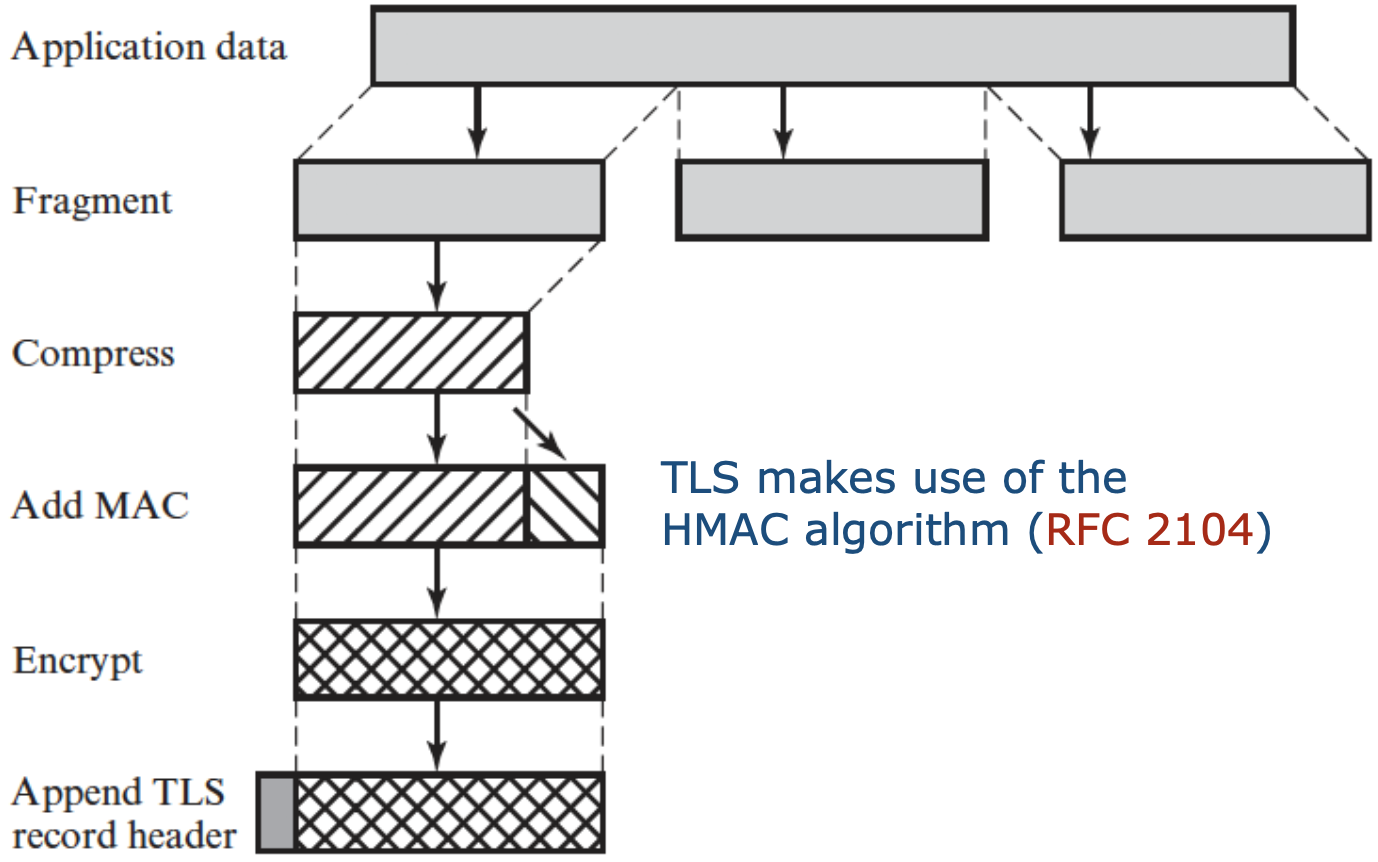
\includegraphics[width=0.7\linewidth]{res/crypto/TLSRecord.png}
\end{figure}
\subsubsection{Change Cipher Spec Protocol}
\textbf{Change Cipher Spec Protocol} consiste in un singolo messaggio, composto da un singolo byte con valore 1. CCS comunica al peer che il mittente vuole scambiare un nuovo set di chiavi, create poi con le informazione scambiate dall'handshake protocol. 
\subsubsection{Alert Protocol}
Alert Protocol è usato per convogliare gli alert di TLS ai pper. Ogni messaggio consiste in due byte, il primo contenente il valore \textit{warning} (1) o \textit{fatal} (2), nel secondo caso terminante la connessione. Il secondo byte contiene un codice che indica l'alert specifico. 
Alcuni esempi possono essere: \verb|unexpected_message|, \verb|bad_record_mac|, \verb|decompression_failure|, \verb|handshake_failure|, \verb|illegal_parameter|.
\subsubsection{Handshake protocol}
Il protocollo di \textbf{handshake} è la parte più complessa di TLS, che permette al server ed al client di autenticarsi a vicenda e negoziare un'encryption, un algoritmo MAC e delle chiavi crittografiche. Viene utilizzato prima di tutto il resto, e ha messaggi $\ge 4$ bytes (1 byte per il type, 3 byte per la lunghezza, ed il payload). Si divide in 4 fasi:
\begin{enumerate}
    \item Stabilire le capabilities di sicurezza
    \item Autenticazione del server e scambio di chiavi 
    \item Autenticazione del client e scambio di chiavi 
    \item Fine
\end{enumerate}
Alcuni messaggi, ad esempio, possono essere \begin{verbatim}
    hello_request, client_hello, server_hello, client_hello, certificate, server_key_exchange,
    certificate_request, server_done, certificate_verify, client_key_exchange, finished
\end{verbatim}. 
Il protocollo supporta più metodi di key exchange, come (EC)DHE, PSK, PSK+ECDHE, un cipher algorithm (AEAD), ed i MAC algorithms basati su HMAC. 
\subsubsection{Heartbeat protocol}
Il protocollo heartbeat è solitamente utilizzato per monitorare la disponibilità di un'entity. Gira sopra TLS Record e consiste di due tipologie di messaggi, \verb|heartbeat request| e \verb|heartbeat response|. Una request può essere inviata sempre, e quando ricevuta richiede una response. Il payload sono dati casuali, poi reinviati nella response per sicurezza.
\subsection{OpenSSL}
OpenSSL è un toolkit robusto per TLS e SSL, includendo anche una libreria general purpose per la crittografia.
\subsection{HTTPS} 
HTTPS significa \textbf{HTTP over SSL/TLS} e si riferisce alla comunicazione basata su HTTP+SSL. Le capacità HTTPS sono presenti in tutti i moderni browser; la porta utilizzata è la 443 e non più la 80. Quando viene usato, sono criptati: l'URL, i contenuti, i forms (POST), i cookies, gli header HTTP. Per HTTPS il client HTTP è anche il client TLS: si svolge prima una TLS connection request, poi TCP connection request. Da qui, si comincia il TLS Handshake ed i dati HTTP vengono inviati come TLS application data. La chiusura della connessione HTTPS richiede che TLS chiuda la connessione con l'entità peer TLS. 
\end{document}
